% This must be in the first 5 lines to tell arXiv to use pdfLaTeX, which is strongly recommended.
\pdfoutput=1
% In particular, the hyperref package requires pdfLaTeX in order to break URLs across lines.

\documentclass[11pt]{article}

% Change "review" to "final" to generate the final (sometimes called camera-ready) version.
% Change to "preprint" to generate a non-anonymous version with page numbers.
\usepackage[preprint]{acl}

% Standard package includes
\usepackage{times}
\usepackage{latexsym}

% For proper rendering and hyphenation of words containing Latin characters (including in bib files)
\usepackage[T1]{fontenc}
% For Vietnamese characters
% \usepackage[T5]{fontenc}
% See https://www.latex-project.org/help/documentation/encguide.pdf for other character sets

% This assumes your files are encoded as UTF8
\usepackage[utf8]{inputenc}

% This is not strictly necessary, and may be commented out,
% but it will improve the layout of the manuscript,
% and will typically save some space.
\usepackage{microtype}

% This is also not strictly necessary, and may be commented out.
% However, it will improve the aesthetics of text in
% the typewriter font.
\usepackage{inconsolata}

%Including images in your LaTeX document requires adding
%additional package(s)
\usepackage{booktabs}
\usepackage{graphicx}
\usepackage{hyperref}

\graphicspath{{images/}}

\title{Emotion Patterns in Reviews of Top-Rated Movies on Letterboxd}

\author{Victor Verma \\
Boston University \\
\texttt{vpverm@bu.edu}}

\begin{document}
\maketitle
\begin{abstract}
We analyze the emotions expressed in user reviews for the highest-rated movies on the social platform Letterboxd. To do so, we introduce the Ekman Emotion Classifier (EEC), a feed-forward neural network trained on the \texttt{Twitter Emotion Corpus} and additional labeled datasets. The model classifies reviews as one of six basic emotions: happiness, sadness, anger, fear, disgust, and surprise. We apply EEC to approximately 70,000 reviews from 65 top-rated movies and uncover emotional patterns. Happiness and sadness are conveyed most frequently, but rarer emotions like disgust and anger are more common in the most-liked reviews. Movies from different decades and countries maintain similar distributions of emotions in their reviews, but movies from different genres have more distinct emotional distributions. These findings offer insight into the emotions evoked by highly rated movies.
\end{abstract}

\section{Introduction}
Letterboxd is a popular social platform which enables users to log, rate, and review movies. On the app, the highest rated movies are grouped in a list called \href{https://letterboxd.com/dave/list/official-top-250-narrative-feature-films/}{Letterboxd's Official Top 250 Narrative Feature Films}, which is updated weekly to reflect new movies and changing ratings \cite{Vis}. We wanted to learn if there were patterns in the emotions that were expressed in reviews for the top-rated movies on the Letterboxd. To explore this, we collected nearly 70,000 reviews from the 65 movies in the list that we had personally seen. \\ \\
Although many pre-trained text-to-emotion classifiers already exist, we decided to build a custom feed-forward neural network, the Ekman Emotion Classifier (EEC). It was trained on the \texttt{Twitter Emotion Corpus (TEC)} and supplementary labeled data found on GitHub \cite{mohammad-2012-emotional, Mohammad, Valente}. The six target emotions were happiness, sadness, anger, fear, disgust, and surprise, inspired by Paul Ekman's work on identifying six basic human emotions \cite{NeuroLaunch}. \\ \\
The first section of this paper describes the unlabeled movie review data to be analyzed, the labeled emotion data used to create the EEC model, and the preprocessing steps that were taken for each dataset. The second section reviews the performance of an existing text-to-emotion classification model to serve as a baseline for the EEC model. The third section summarizes the performance of our model, focusing on key metrics such as precision, recall, and F1-score, the standard for multiclass classification tasks. The last section identifies patterns in the emotions expressed by users by applying the EEC model to the Letterboxd movie review dataset. \\ \\
It was found that happiness and sadness were the most common emotions, while disgust and anger were the least common. On average, the most liked reviews tended to be those expressing the least common emotions, and vice versa. The approximate distribution of emotions in reviews remained the same regardless of the release decade of the movie or the country the movie was from, but changed depending on its genre.
\section{Data}
\subsection{Letterboxd Movie Reviews}
The movie review data was sourced from Letterboxd's Official Top 250 Narrative Feature Films list \cite{Vis}. Although the list contains 250 movies, reviews were only retrieved from the 65 that we had seen at the time of collection. The official list is updated weekly, but the gathered data is from the version on February 24th, 2024. \\ \\
For each movie, the first 1,200 reviews sorted in order of decreasing activity were scraped. Each individual review was organized as a JSON object containing the author's rating of the movie, the date of the review, the number of comments left on the review, the review text, and the number of likes the review received. These were then aggregated in CSV files with each field as a column. \\ \\
Several steps were taken to preprocess the movie review data. First, all of the \texttt{None} and \texttt{NaN} reviews were dropped. Next, the emojis in the review text were converted into their textual equivalent. Non-English language reviews were then removed for convenience, as well of those solely consisting of punctuation. Finally, unnecessary whitespaces and newline characters were deleted to minimize the length of each review. \\ \\
The processed dataset contained 65,967 movie reviews, with each receiving 153 likes and 3 comments on average. The distribution of ratings given by the user to the movie being reviewed, measured on scale of 0.5 - 5.0, is summarized in \hyperref[tab:review_rating_distribution]{Table 2.1.1}. Most of the ratings associated with reviews were high, which was expected given that the reviews were taken from the top-rated movies on Letterboxd. This led to the expectation that positive emotions would be expressed most often.
\renewcommand{\thetable}{2.1.1}
\begin{table}[h]
    	\centering
    	\begin{tabular}{c c c}
        		\toprule
        		\textbf{Rating} & \textbf{Number of Reviews} & \textbf{Percentage} \\
        		\midrule
        		None & 1,858 & 2.82\% \\
        		0.5 & 400 & 0.61\% \\
        		1.0 & 237 & 0.36\% \\
        		1.5 & 132 & 0.20\% \\
        		2.0 & 366 & 0.56\% \\
        		2.5 & 471 & 0.72\% \\
        		3.0 & 1,209 & 1.83\% \\
        		3.5 & 2,329 & 3.54\% \\
        		4.0 & 8,586 & 13.05\% \\
        		4.5 & 13,589 & 20.65\% \\
        		5.0 & 36,321 & 55.20\% \\
        		\bottomrule
    	\end{tabular}
    	\caption{Distribution of Movie Ratings}
    	\label{tab:review_rating_distribution}
\end{table}
\subsection{Twitter Emotion Corpus}
The initial training data for the EEC model was sourced from the \texttt{Twitter Emotion Corpus (TEC)} \cite{mohammad-2012-emotional, Mohammad}. The raw \texttt{.txt} file was parsed into a CSV with the text and emotion label as columns, and preprocessed in a similar manner to the movie review data. First, the emojis were converted into their textual equivalent. Next, non-English language and punctuation-only reviews were removed. Finally, unnecessary whitespaces and newline characters were deleted. \\ \\
The processed \texttt{TEC} dataset consisted of 19,333 text-label pairs, and the distribution of labels is shown in \hyperref[tab:emotion_label_distribution]{Table 2.2.1}. It would have been ideal to have an equal number of observations for each emotion class, but no such dataset was found.
\renewcommand{\thetable}{2.2.1}
\begin{table}[h]
    	\centering
    	\begin{tabular}{c c c}
        		\toprule
        		\textbf{Class} & \textbf{Count} & \textbf{Percentage} \\
        		\midrule
        		Happiness & 7,892 & 40.82\% \\
        		Sadness & 3,613 & 18.69\% \\
        		Anger & 1,489 & 7.70\% \\
        		Fear & 2,563 & 13.28\% \\
        		Disgust & 733 & 3.79\% \\
        		Surprise & 3,043 & 15.74\% \\
        		\bottomrule
    	\end{tabular}
    	\caption{TEC Emotion Class Distribution}
	\label{tab:emotion_label_distribution}
\end{table}
\subsection{Combined Emotion Data}
In practice, it was found that using only the \texttt{TEC} dataset to train the EEC model resulted in a low macro F1-score. Furthermore, the class imbalance increased the variance of the prediction accuracy across emotion classes. To improve classification performance, supplementary labeled data was found on GitHub \cite{Valente}. The additional data was merged with the \texttt{TEC} data to create a combined dataset containing 36,464 text-label pairs, whose label distribution is shown in \hyperref[tab:combined_emotion_label_distribution]{Table 2.3.1}. The class imbalance remained an issue, but with a lack of publicly available labeled data, the model was forced to make do with what it had.
\renewcommand{\thetable}{2.3.1}
\begin{table}[h]
    	\centering
    	\begin{tabular}{c c c}
        		\toprule
        		\textbf{Label} & \textbf{Count} & \textbf{Percentage} \\
        		\midrule
        		Happiness & 14,264 & 39.12\% \\
        		Sadness & 8,918 & 24.46\% \\
        		Anger & 4,025 & 11.04\% \\
        		Fear & 4,798 & 13.16\% \\
        		Disgust & 733 & 2.01\% \\
        		Surprise & 3,726 & 10.22\% \\
        		\bottomrule
    	\end{tabular}
    	\caption{Combined Emotion Class Distribution}
	\label{tab:combined_emotion_label_distribution}
\end{table}

\section{Baseline}
Initial emotion class inference was completed using a baseline Ekman Classifier model from Hugging Face. It was built using the \texttt{BERT} architecture, finetuned using Google's \texttt{GoEmotions} dataset, and classifies text as one of the six Ekman emotions \cite{Ghoshal, Ghoshal2, demszky2020goemotions}. The baseline model only achieved a macro F1-score of 0.39 on the combined emotion dataset, much lower than expected from a pre-trained model. \\ \\
The precision, recall, and F1-score for each emotion class are summarized in \hyperref[tab:baseline_summary_statistics]{Table 3.1}. Only three out of six emotions, happiness, sadness, and fear, had a precision greater than 0.50. This suggested that the baseline model produced a large number of false positives. Only happiness had a recall greater than 0.50, which indicated that the baseline model also produced a large number of false negatives. Consequently, only happiness and sadness had F1-scores greater than 0.50, confirming that the baseline model was objectively bad at identifying the Ekman emotions.
\renewcommand{\thetable}{3.1}
\begin{table}[h]
    	\centering
    	\begin{tabular}{c c c c}
        		\toprule
        		\textbf{Emotion} & \textbf{Precision} & \textbf{Recall} & \textbf{F1-Score} \\
        		\midrule
        		Happiness & 0.60 & 0.78 & 0.68 \\
        		Sadness & 0.65 & 0.47 & 0.54 \\
        		Anger & 0.40 & 0.44 & 0.42 \\
        		Fear & 0.63 & 0.26 & 0.37 \\
        		Disgust & 0.09 & 0.09 & 0.09 \\
        		Surprise & 0.23 & 0.30 & 0.26 \\
        		\bottomrule
    	\end{tabular}
    	\caption{Baseline Model Performance Statistics}
	\label{tab:baseline_summary_statistics}
\end{table}
\\ \\ The failures of the baseline model were further investigated using the confusion matrix displayed in \hyperref[fig:baseline_confusion_matrix_combined]{Figure 3.2}, which offered insight into how emotions were being labeled. For example, it was found that happiness was most commonly mislabeled as sadness, an unexpected result since the emotions are semantically opposite. Another observation is that text conveying surprise was mislabeled as happiness twice as often as it was labeled correctly. The model had a hard time classifying anger, fear, and disgust, likely due to the lack of training data for those classes. Overall, the baseline model served as a good starting point but did not work as well as expected.
\renewcommand{\thefigure}{3.2}
\begin{figure}[h]
	\centering
	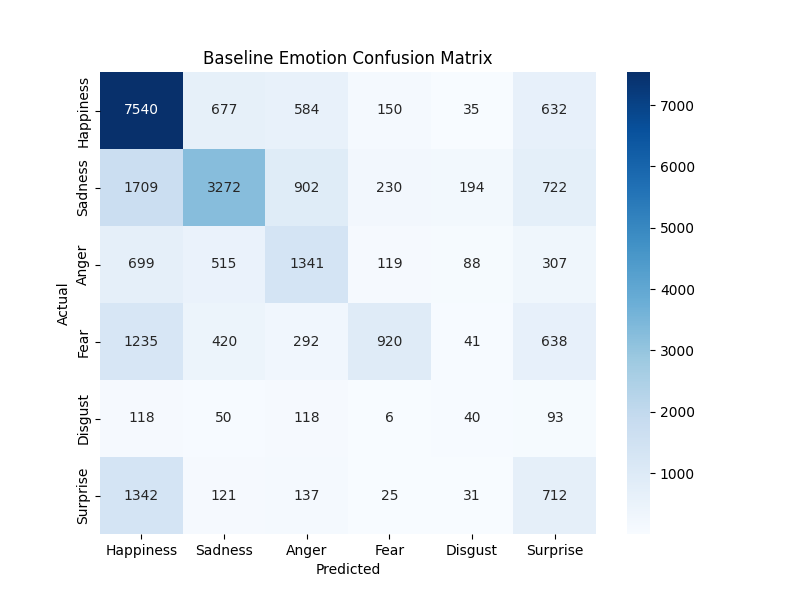
\includegraphics[width=0.45\textwidth]{baseline_emotion_confusion_matrix_combined.png}
	\caption{Baseline Model Confusion Matrix}
	\label{fig:baseline_confusion_matrix_combined}
\end{figure}

\section{Models}
\subsection{Architecture}
A custom feed-forward neural network was designed to perform multiclass emotion classification. The Ekman Emotion Classifer (EEC) model architecture is shown in \hyperref[fig:eec_architecture]{Figure 4.1.1}. The input layer takes in a 384-dimensional vector embedding of the text to be classified, which is then passed through a fully connected (linear) layer with 256 hidden units. The ReLU activation function is applied to the output of the first linear layer, and the result is passed through a second linear layer. The latter maps the 256-dimensional hidden representation to a 6-dimensional output (corresponding to the six target classes).
\renewcommand{\thefigure}{4.1.1}
\begin{figure}[h]
	\centering
	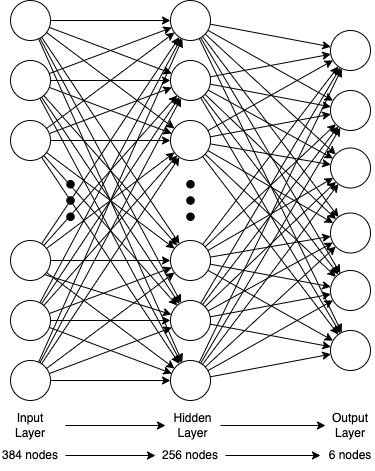
\includegraphics[width=0.33\textwidth]{eec_architecture.png}
	\caption{EEC Architecture}
	\label{fig:eec_architecture}
\end{figure}
\\ \\ Experiments were conducted varying both the size of the hidden layer and the number of hidden layers, and the current configuration was chosen because it produced the best results.
\subsection{Text Embedding Model}
The input layer for the classification model could be configured to ingest any n-dimensional vector. During development, two popular text embedding models were selected from Hugging Face. \\ \\
The \texttt{sentence-transformers/all-MiniLM-L6-v2} embedding model maps text to a dense 384-dimensional vector that captures semantic information. It is intended for sentences and short paragraphs, which made it ideal for both the training data and its application in classifying movie reviews \cite{all-MiniLM-L6-v2}. \\ \\
The \texttt{moka-ai/m3e-base} embedding model encodes 768-dimensional vectors, and it was chosen because it had the most likes of any text embedding model on Hugging Face \cite{MokaMassiveMixedEmbedding}. \\ \\
While using embeddings generated by the \texttt{sentence-transformers/all-MiniLM-L6-v2} model, the best classification model achieved a macro F1-score of 0.57 on the validation dataset. This was slightly higher than the 0.50 macro F1-score reached using \texttt{moka-ai/m3e-base} embeddings on the same dataset. Consequently, the former text embedding model was used in the EEC model.
\subsection{Neural Model}
The neural component of the EEC model consisted of the aforementioned feed-forward neural network, shown in  \hyperref[fig:eec_architecture]{Figure 4.1.1}. The input layer was configured to have 384 nodes to match the 384-dimensional vector embeddings produced by the \texttt{sentence-transformers/all-MiniLM-L6-v2} model. The model was trained used cross-entropy loss, common for multiclass classification tasks, and further optimized by using stochastic gradient descent with momentum. \\ \\
There were four parameters to configure during training: the learning rate, the momentum, the number of epochs, and the batch size. During development, grid searches were conducted over the combinations of training datasets, embedding models, and training parameters. The EEC model was produced by using the combined emotion dataset with the \texttt{sentence-transformers/all-MiniLM-L6-v2} embeddings. This model was trained for 100 epochs using a learning rate of 0.01, momentum of 0.9, and batch size of 64. \\ \\
To visualize the effectiveness of the training parameter configuration, the training loss was plotted as a function of epoch. In \hyperref[fig:training_loss]{Figure 4.3.1}, the training loss over time for the EEC model is shown with a logarithmic y-scale for clarity while displaying small values. From the curve, it can be seen that there is an initial rapid decrease in loss followed by a slower rate of decline. The nearly linear curve by the end of training indicates exponential decay, suggesting that training should be stopped to avoid overfitting.
\renewcommand{\thefigure}{4.3.1}
\begin{figure}[h]
	\centering
	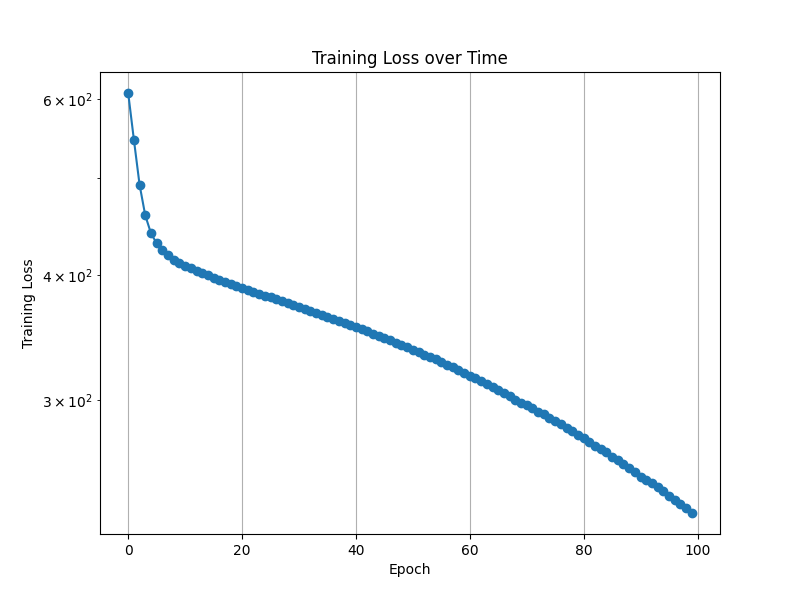
\includegraphics[width=0.45\textwidth]{training_loss.png}
	\caption{Training Loss}
	\label{fig:training_loss}
\end{figure}
\\ \\ To further ensure proper model training, the F1-scores of the test and validation sets were compared. For the EEC model, the macro F1-score of the test set was approximately 0.55, and the macro F1-score of the validation set was about 0.57. The closeness of these values was a strong indicator that the model was appropriately trained.
\subsection{Model Performance}
The performance of the EEC model was evaluated using the precision, recall, and F1-scores on the validation set, shown in  \hyperref[tab:eec_summary_statistics]{Table 4.4.1}. The macro F1-score was 0.57, a 0.18 point increase from the baseline model's 0.39. There was also an improvement across every class' individual F1-score, with the biggest increase for disgust with a 0.30 point jump.
\renewcommand{\thetable}{4.4.1}
\begin{table}[h]
    	\centering
    	\begin{tabular}{c c c c}
        		\toprule
        		\textbf{Emotion} & \textbf{Precision} & \textbf{Recall} & \textbf{F1-Score} \\
        		\midrule
        		Happiness & 0.75 & 0.76 & 0.76 \\
        		Sadness & 0.58 & 0.77 & 0.66 \\
        		Anger & 0.61 & 0.46 & 0.53 \\
        		Fear & 0.66 & 0.62 & 0.64 \\
        		Disgust & 0.49 & 0.32 & 0.39 \\
        		Surprise & 0.57 & 0.36 & 0.44 \\
        		\bottomrule
    	\end{tabular}
    	\caption{EEC Model Performance Statistics}
	\label{tab:eec_summary_statistics}
\end{table}
\\ \\ The confusion matrix of the predicted classes on the validation set is shown in \hyperref[fig:eec_model_confusion_matrix]{Figure 4.4.2}. Disgust was regularly misclassified, and there remained confusion between surprise and happiness. This variance was expected due to the imbalanced training dataset.
\renewcommand{\thefigure}{4.4.2}
\begin{figure}[h]
	\centering
	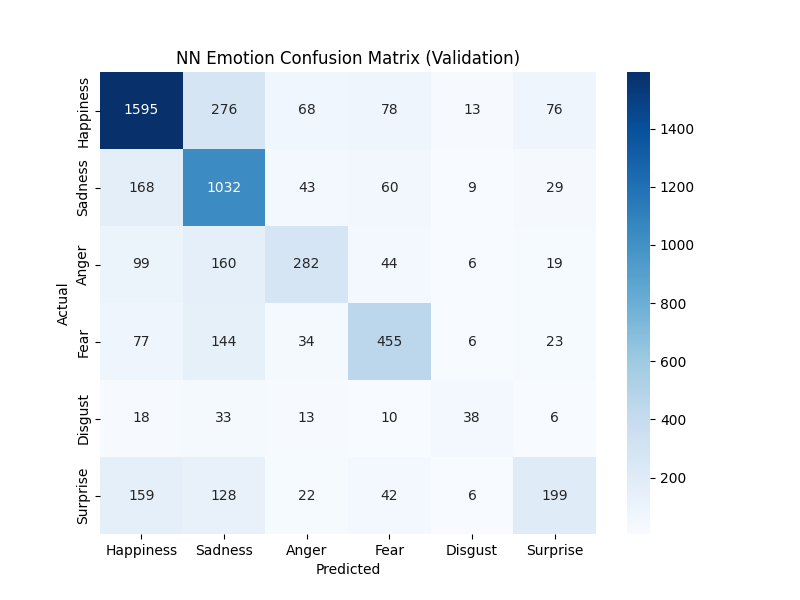
\includegraphics[width=0.45\textwidth]{validation_nn_emotion_confusion_matrix_combined.png}
	\caption{EEC Model Confusion Matrix}
	\label{fig:eec_model_confusion_matrix}
\end{figure}
\section{Classifying Movie Reviews}
The EEC model was used to classify the emotions expressed in the movie review dataset, a collection of 65,967 reviews gathered from top-rated movies on Letterboxd. The distribution of emotions expressed in the reviews is shown in \hyperref[tab:movie_review_distribution]{Table 5.1}.  \\ \\
As expected, happiness was the most prevalent emotion, expressed in nearly 37\% of all reviews. Sadness was the second most common emotion, which also makes sense because a lot of highly rated movies are based on true or important stories that are reflective of life, which naturally contain an element of sadness. The least frequent emotions were disgust and anger, combining for less than 8\% of reviews.
\renewcommand{\thetable}{5.1}
\begin{table}[h]
    	\centering
    	\begin{tabular}{c c c}
        		\toprule
        		\textbf{Emotion} & \textbf{Count} & \textbf{Percentage} \\
        		\midrule
        		Happiness & 24,404 & 36.99\% \\
        		Sadness & 17,924 & 27.17\% \\
        		Anger & 4,261 & 6.46\% \\
        		Fear & 12,754 & 19.33\% \\
        		Disgust & 633 & 0.96\% \\
        		Surprise & 5,991 & 9.08\% \\
        		\bottomrule
    	\end{tabular}
    	\caption{Distribution of Emotions in Movie Reviews}
	\label{tab:movie_review_distribution}
\end{table}
\\ \\ Beyond the raw counts, the emotions expressed in reviews were stratified across different categories to identify less obvious patterns. In \hyperref[fig:emotion_counts_by_release_decade]{Figure 5.2}, reviews were grouped by the release decade of the associated movie. Interestingly, it was found that the distribution of emotions expressed in reviews was approximately the same across all nine decades being compared.
\renewcommand{\thefigure}{5.2}
\begin{figure}[h]
	\centering
	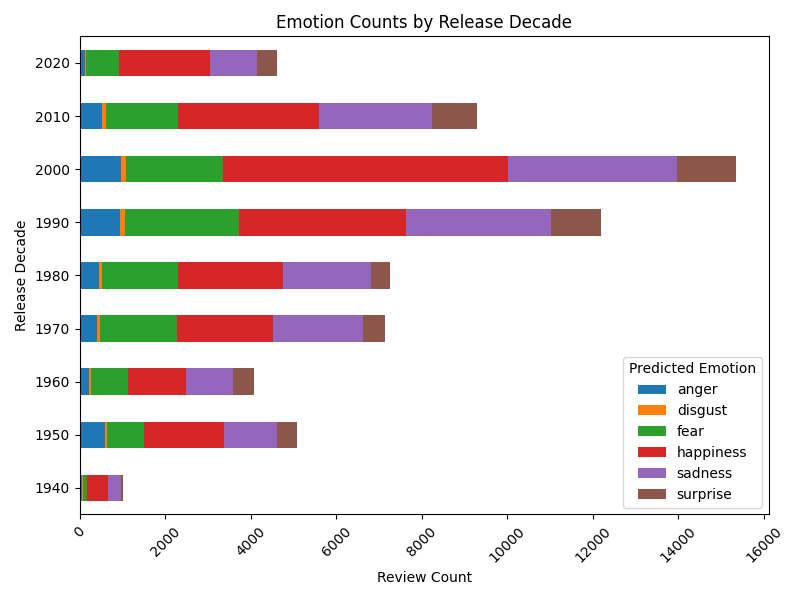
\includegraphics[width=0.45\textwidth]{emotion_counts_by_release_decade.png}
	\caption{Emotion Counts by Release Decade}
	\label{fig:emotion_counts_by_release_decade}
\end{figure}
\\ \\ In \hyperref[fig:emotion_counts_by_country]{Figure 5.3}, movies were stratified by the country from which they originated. Again, it was observed that the distribution of emotions in reviews remained nearly identical to the overall distribution.
\renewcommand{\thefigure}{5.3}
\begin{figure}[h]
	\centering
	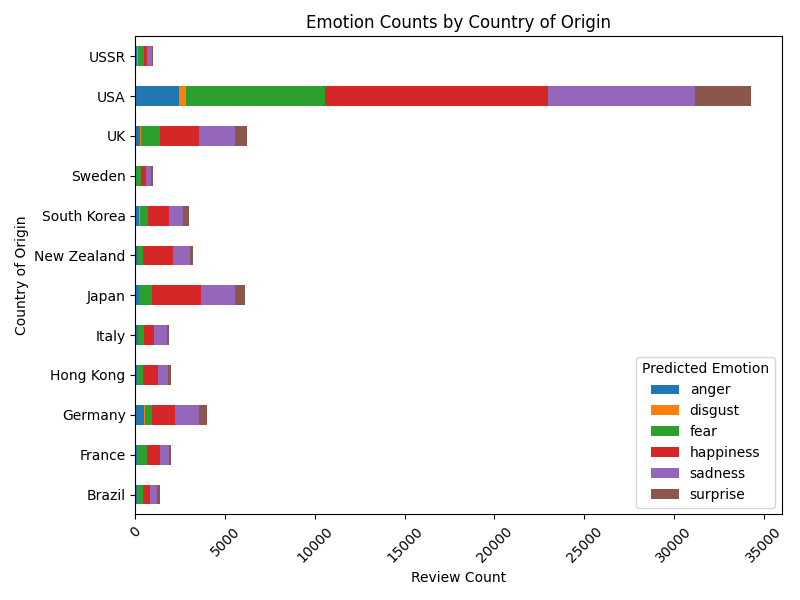
\includegraphics[width=0.45\textwidth]{emotion_counts_by_country.png}
	\caption{Emotion Counts by Country of Origin}
	\label{fig:emotion_counts_by_country}
\end{figure}
\\ \\ In \hyperref[fig:emotion_counts_by_genre]{Figure 5.4}, movies were grouped by their genre, and for the first time, there was a noticeable difference in the distribution of emotions. The most frequent emotion in horror movie reviews was fear, and the most common emotion in history movie reviews was sadness. Meanwhile, a relatively high percentage of reviews for both thriller and mystery movies expressed surprise.
\renewcommand{\thefigure}{5.4}
\begin{figure}[h]
	\centering
	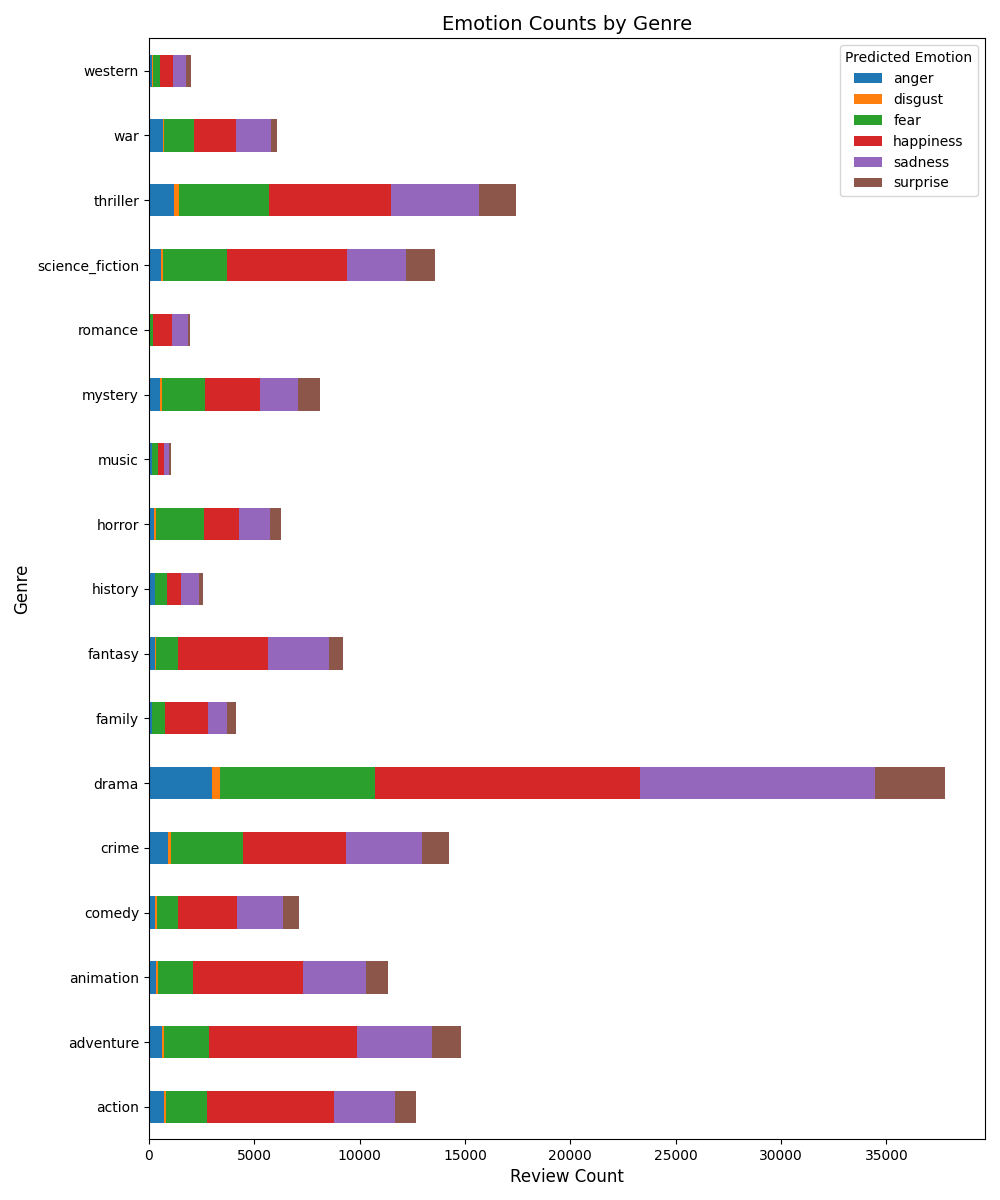
\includegraphics[width=0.45\textwidth]{emotion_counts_by_genre.png}
	\caption{Emotion Counts by Genre}
	\label{fig:emotion_counts_by_genre}
\end{figure}
\\ \\ On Letterboxd, users are also able to like reviews. To take this feature into consideration, the average number of likes per emotion was calculated, as shown in \hyperref[fig:average_likes_per_emotion]{Figure 5.5}. An unexpected trend emerged: the reviews expressing the least frequent emotions received the most likes on average, and vice versa. It is unclear why this pattern developed, but it could be worth investigating further.
\renewcommand{\thefigure}{5.5}
\begin{figure}[h]
	\centering
	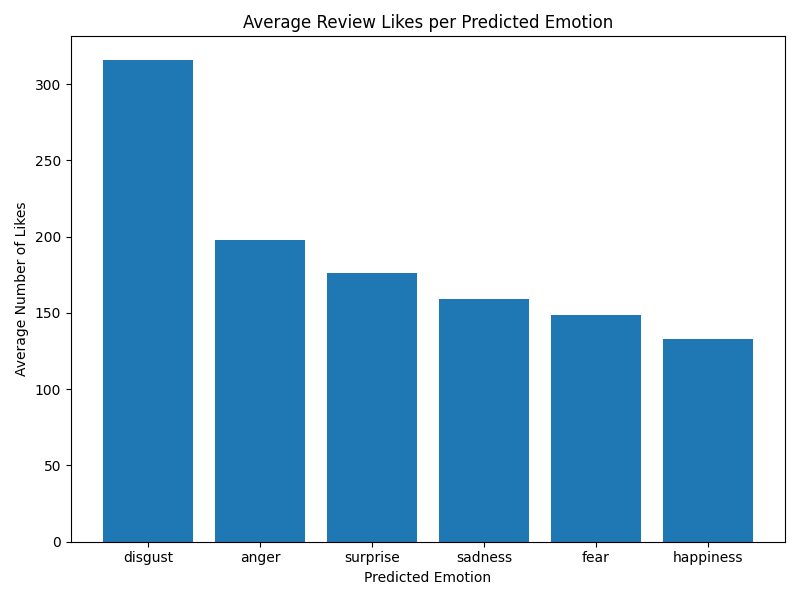
\includegraphics[width=0.45\textwidth]{average_likes_per_emotion.png}
	\caption{Average Review Likes per Emotion}
	\label{fig:average_likes_per_emotion}
\end{figure}
\section{Conclusion}
In this paper, we developed the Ekman Emotion Classifier (EEC), a feed-forward neural network trained to identify the six basic Ekman emotions from text. We used the EEC model to find patterns in the emotions expressed in nearly 70,000 movie reviews from 65 of the highest rated movies on the Letterboxd social platform. \\ \\
Our analysis revealed that reviews most frequently conveyed happiness and sadness, but rarer emotions like disgust and anger tended to receive more likes on average. The distribution of emotions expressed in reviews remained similar for movies released in different decades or originating from different countries, but varied across genres. These findings offer unique insight into the emotional impact that top-rated movies can have on their audience.
\section{Limitations}
The biggest limitation in this work came from the imbalanced training dataset for the EEC model. The lack of labeled observations for disgust and surprise particularly hurt model performance and decreased the macro F1-score. The batch size during training was made several times greater than the imbalance ratio to mitigate the issue, but techniques such as downsampling and upweighting were not implemented \cite{Imbalanced}. \\ \\
The development of the neural network architecture was inherently constrained by time and compute resources. Each grid search for training parameters only checked 48 combinations due to these limitations, far less than the several thousand that were originally proposed. It would also have been ideal to experiment with additional configurations of hidden layers and sizes.
\section{Future Work}
The conclusions from this paper were made using a custom emotion classification model specially designed to identify the six Ekman emotions from text. The results should be independently verified using a state-of-the-art classification model. \\ \\
The emotion patterns can be further generalized by increasing both the total number of reviews and the number of movies that are included in the movie review dataset.
\section{Acknowledgements}
We thank Professor Andrew Wood for his guidance and Boston University for the opportunity to complete this research through CS505.
\bibstyle{acl_natbib}
\bibliography{custom}

\end{document}
